\documentclass{cosas/tfg_domingo}
% \documentclass[numeros]{tfg_domingo}

\autor{Alejandro Martínez Floranes}
\titulo{Reescribir Slatt en python 3}
% Título corto para los encabezamientos de pagina:
\corto{} % En blanco si no es necesario recortarlo.
\ingles{Rewrite Slatt in python 3}
\fecha{julio de 2021}
% La normativa prescribe «cuatro o cinco palabras clave, en
% español y en inglés, para su indexación en el repositorio
% de TFG».
\palabras{reglas de asociación, hipergrafos, Slatt, refactorizar}%
  {association rules, hypergraph, Slatt, refactor}

\usepackage{lipsum} % Esto solo es relleno.
\usepackage{listings}
\usepackage{xcolor}
\usepackage{amssymb}
\usepackage{multirow}

\definecolor{codegreen}{rgb}{0,0.6,0}
\definecolor{codegray}{rgb}{0.5,0.5,0.5}
\definecolor{codepurple}{rgb}{0.58,0,0.82}
\definecolor{backcolour}{rgb}{0.95,0.95,0.92}

\lstdefinestyle{mystyle}{
    %backgroundcolor=\color{backcolour},   
    commentstyle=\color{codegreen},
    keywordstyle=\color{magenta},
    numberstyle=\tiny\color{codegray},
    stringstyle=\color{codepurple},
    basicstyle=\ttfamily\footnotesize,
    breakatwhitespace=false,         
    breaklines=true,                 
    captionpos=b,                    
    keepspaces=true,                 
    numbers=left,                    
    numbersep=5pt,                  
    showspaces=false,                
    showstringspaces=false,
    showtabs=false,                  
    tabsize=2
}

\lstset{style=mystyle}

\begin{document}

% Si alguna palabra se divide entre dos líneas en un punto
% indebido, podemos indicar aquí los puntos de corte
% aceptables (si los hay), p. ej,
% \hyphenation{ba-rro-co, frío, cria-do, su-per-ra-tón}
\hyphenation{Dijkstra new-speak}

\portada
\frontmatter
% \sucinto{A Sofía}
\gracias{\input{cosas/agradecimientos.txt}}
\resumen{Las reglas de asociación son objetos matemáticos empleados de forma extensa en disciplinas como la minería de datos, aprendizaje automático y representación del conocimiento, entre otros campos.
Slatt es un proyecto de software libre desarrollado por José Luis Balcázar (Universidad Politécnica de Barcelona). Ofrece funcionalidades para el cálculo de reglas de asociación. Para ello, se apoya en implementaciones del algoritmo a priori para el cálculo de clausuras, el retículo de las clausuras y, entre otras
funcionalidades,devuelve las reglas representativas para cualquier elección de los parámetros de soporte y confianza.

En este proyecto, se ha mejorado este software utilizando como base las implementaciones disponibles en Slatt aplicadas a:

\begin{itemize}
    \item hipergrafos y algoritmos con aplicación a estos objetos;
    
    \item cálculo de clausuras y retículos (lattices);
\end{itemize}


Este trabajo ha requerido la búsqueda y análisis de algoritmos propuestos en la literatura científica sobre los puntos anteriores.
El lenguaje de desarrollo será Python3, encontrándose la implementación anterior en Python 2.7
%
% Conviene evitar aquí las llamadas a la bibliografía del
% trabajo, ya que el resumen tiene entidad independiente.
%

%% Aportamos nuestra perspectiva sobre la pertinencia de las
%% instrucciones {\tt goto}.


%%Pasar a tiempo presente
}{Association rules are mathematical objects used extensively in disciplines such as data mining, machine learning, and knowledge representation, among other fields.
Slatt is a free software project developed by José Luis Balcázar (Polytechnic University of Barcelona). It offers functionalities for the calculation of association rules. To do this, it relies on implementations of the a priori algorithm for the calculation of closures, the lattice of closures and, among others
functionalities, returns the representative rules for any choice of support and trust parameters.

In this project, this software has been improved using as a basis the implementations available in Slatt applied to:

\begin{itemize}
    \item hypergraphs and algorithms with application to these objects;
    
    \item calculation of closures and lattices (lattices);
\end{itemize}


This work has required the search and analysis of algorithms proposed in the scientific literature on the previous points.
The development language will be Python3, the previous implementation being in Python 2.7
}
\tableofcontents

\mainmatter
\chapter{\emph{Introducción}}

\section{Minería de datos}
La minería de datos es un área de investigación cuyo objetivo de extraer información de grandes volúmenes de datos.
Sus aplicaciones cubren diversas áreas y emplean técnicas de estadística, ciencias de la computación y bases de datos. Con la masificación de datos se ha convertido en un problema para un humano controlar y manejar esta información, por ello es necesario resumir e identificar esta información para mostrarle al usuario de forma concisa.
Entre todos estas técnicas que se utilizan, una de las diez más importantes son las reglas de asociación como se menciona en el artículo de \citet{wu2008top}.
Encontrar estas reglas no es sencillo, el primer algoritmo de reglas de asociación fue dado por  \citet{agrawal1993mining}, pero sufría por una costosa complejidad computacional.
A partir de este algoritmo, se propuso el algoritmo Apriori en el artículo  \citet{agrawal1994fast}.
Desafortunadamente, el algoritmo Apriori también tiene sus limitaciones ya que genera muchas reglas redundantes, es decir, que tienen la misma significación o que se derivan unas de otras. Esto a generado interés entre los investigadores para minimizar el numero de reglas de asociación sin perder información valiosa para el usuario. \par

Una de las primeras formas de medir la redundancia entre reglas de asociación fue dado en \citep{kryszkiewicz2001closed}. Donde la idea principal es que una regla no aporta información a un usuario si es consecuencia lógica de otra regla.
Hay muchas librerías y programas que implementan algoritmos para hallar reglas de asociación con la mínima redundancia posible, entre ellas Slatt, que ha sido usada en varios artículos \citep{balcazar2010closure, tirnuaucua2020closed} y otros artículos relacionados con las reglas de asociación.

Actualmente, el desarrollo de la librería Slatt muestra ciertas carencias : esta programada en una versión antigua de python, en concreto en python 2.7, tiene dentro de ella 13 clases de las cuales más de la mitad poseen código repetido y un número de lineas de código excesivas para la funcionalidad que esta librería proporciona.
El cometido principal de este proyecto es mejorar la lectura y rendimiento del código, eliminando código repetido y añadiendo diversas funcionalidades que nos entrega python 3.x como es la metaprogramación.

\section{Reglas de asociación}

Unos de los objetivos de este proyecto es actualizar Slatt a python 3, aprovechar las posibilidades que nos brinda la metaprogramación e incluir diferentes mejoras en el código para mejorar tanto su eficiencia en cuanto a rendimiento, como en reducción de lineas de código sin empeorar la legibilidad del mismo.

\hfill

Las mejoras que se han hecho en Slatt se han incorporado en un repositorio abierto, ya que la licencia de Slatt es libre.

\hfill

Una base de datos esta formada por \textbf{transacciones}  conjunto de órdenes que se ejecutan formando una unidad de trabajo, \textbf{items} archivos informáticos que contiene datos sobre un dataset  y \textbf{conjuntos de items} conjunto de uno o más items que permiten en el caso de las reglas de asociación calcular diferentes parámetros como son la cobertura o el soporte.


Las reglas de asociación son expresiones del tipo $W \rightarrow B$ donde $W, B \subset I$. El significado es que en las transacciones de la base de datos que tienen los items de $W$ tienden a tener los items en el conjunto $B$.. Los parámetros esenciales para comparar las reglas de asociación son: \textit{el soporte, la confianza y el lift.} \ref{asoc_rules}

\begin{figure}[ht!] % [h!] fuerza que el elemento se sitúe
                    % en la posición señalada, en vez de al
                    % comienzo de una página.
\begin{center}
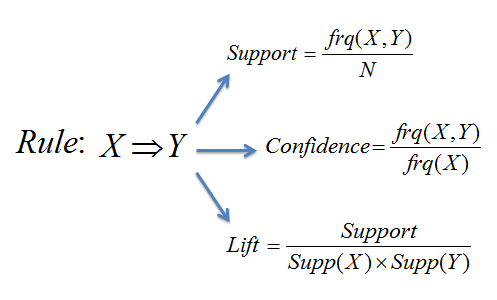
\includegraphics[width=.49\linewidth]{imagenes/AR_1.png}
\end{center}
\caption{Association Rules}
\label{asoc_rules}
\end{figure}

\begin{itemize}
    \item El \textbf{frq(X,Y)} es las frecuencia de que aparezca el item X y el item Y en una misma transacción.
    \item El \textbf{soporte} es la fracción de las transacciones que contiene tanto a X como a Y. 
    \item La \textbf{confianza} es la fracción de las transacciones en las que aparece X que también incluyen a Y; esto es, la confianza mide con que frecuencia aparece Y en las transacciones que incluyen X.
    \item El \textbf{lift} es la confianza de la reglas dividido por el cociente del consecuente.
\end{itemize}

A su vez, a la hora de plantear un problema utilizando reglas de asociación necesitamos disponer de diferentes elementos:  

\begin{enumerate}
    \item \textbf{Itemset.- } Conjunto de uno o más items $X, Y$.
    \item \textbf{K-itemset.- } Itemset con k elementos.
    \item \textbf{Soporte de un itemset.- } Fracción de las transacciones que contienen el itemset.
    \textbf{Itemset Frecuente} Itemset con soporte igual o superior a un umbral de soporte establecido por el usuario. 
    \item \textbf{Umbral mínimo de confianza y de soporte.- } estos umbrales se utilizan para coger las reglas cuyo soporte o confianza sean mayores que las de umbral mínimo.
\end{enumerate}

Para dar los ejemplos nos apoyamos seguiremos los ejemplos clásicos dados por \citep{agrawal1993mining}, donde consideran el problema de la cesta de la compra. Este problema da una base datos con diferentes items y transacciones que representan las compras de varias personas en un supermercado a lo largo de un cierto tiempo. El objetivo es llegar a conocer los patrones de comportamiento a la hora de realizar la lista de la compra.
En el cuadro \ref{prob_asoc} se muestra un ejemplo sencillo de una instancia del problema de la lista de la compra (\citet{datamining}).
\newpage

\begin{table}[h]
\centering
\begin{tabular}{|l|l|l|}
\hline
TID & Artículos                     \\ \hline
1         & Pan, leche, huevos            \\ \hline
2         & Pan, pañales, cerveza            \\ \hline
3         & Leche, pañales, cerveza            \\ \hline
4         & Pan, leche, pañales, cerveza         \\ \hline
5         & Pan, leche, huevos, cerveza         \\ \hline
\end{tabular}
\caption{Problema reglas de asociación}
\label{prob_asoc}
\end{table}

\begin{tcolorbox}[colback=red!5!white,colframe=red!75!black]
  \textbf{Ejemplo de calculo sobre la Tabla} \ref{prob_asoc}

  El \textbf{soporte} de la cerveza, supp(cerveza) = 4/5 = 0.8
  
  El \textbf{soporte} de los pañales, supp(pañales) = 3/5 = 0.6
  
  El \textbf{soporte} de la cerveza y los pañales, supp(cerveza,pañales) = 3/5 = 0.6
  
  La \textbf{confianza} entre la cerveza y los pañales seria, supp(cerveza,pañales) / supp(cerveza) = 0.6 / 0.8 = 0.75
  
\end{tcolorbox}

Para implementar este tipo de operaciones en código python, Slatt usa el algoritmo Apriori para recuperar los itemsets cuyo soporte sea mayor que un valor dado. Para resolver este problema de enumeración, Apriori utiliza una exploración en anchura entre todos los itemsets de la siguiente forma: \citep{aggarwal2015data}

\begin{enumerate}
    \item Genera los itemsets.
    \begin{itemize}
        \item Genera todos los itemsets con un elemento.
        \item Usa estos para generar los de dos elementos, y así sucesivamente.
        \item Toma todos los que cumplen con el mínimo soporte (esto permite eliminar posibles combinaciones).
    \end{itemize}
    \item Genera las reglas revisando que cumplan con el criterio mínimo de confianza.
\end{enumerate}

\lstinputlisting[language=python,caption=\textbf{Apriori Algorithm python version},frame=bottom]{codigo/apriori.py}




% Utilice «citet» para integrar el nombre del autor en el
% texto. Para referencias aisladas, «citep».

\newpage
\section{Metodología y Requisitos}

Debido a la extensión de este proyecto, se decidió usar una metodología incremental en la segunda reunión de tutoría ya que dicho proyecto posee una gran carga teórica.

Las reuniones se realizaban de manera semanal o cada dos semanas, dependiendo de las dudas que me fuesen surgiendo durante dichas semanas sobre que poder introducir en el código o que tipo de estructuras de datos nueva utilizar, etc. A la entrada de la reunión se leía que se había discutido la semana anterior, se le daba una explicación al tutor de las dudas y los cambios que había estado realizando esas últimas semanas y se empezaba a revisarlo.

Se ha tenido siempre una versión la cual íbamos cambiando, se empezó con la versión antigua de Slatt y siempre que se realizaba algún cambio en el código, se comprobaba que las salidas de código de la versión antigua y la modificada fuesen iguales usando tests unitarios. Esto se discutirá en el último capítulo. 



\begin{figure}[ht!] % [h!] fuerza que el elemento se sitúe
                    % en la posición señalada, en vez de al
                    % comienzo de una página.
\begin{center}
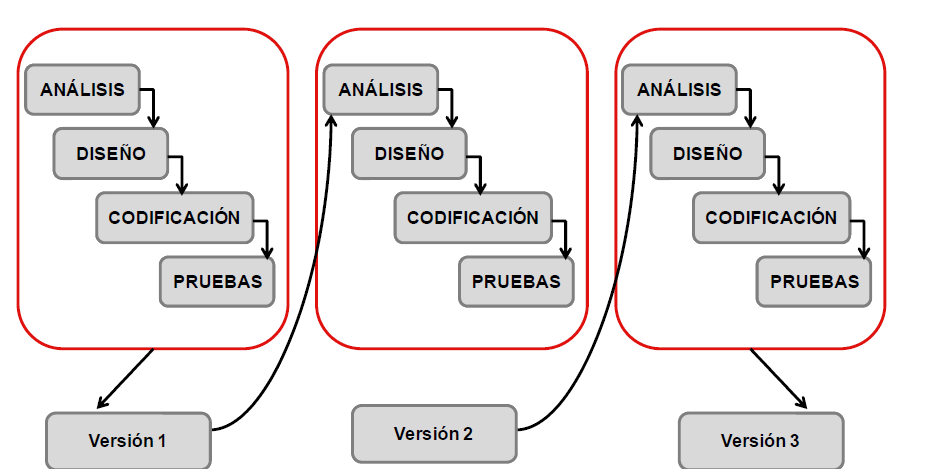
\includegraphics[width=.7\linewidth]{imagenes/Metodologia.png}
\end{center}
\caption{Metodología iterativa incremental}
\label{fig_pro}
\end{figure}

A continuación, defino los requisitos no funcionales del proyecto software, al no ser una aplicación destinada hacia un usuario (cliente) al uso, los requisitos no funcionales, se basan en el correcto funcionamiento de la aplicación.

\begin{table}[h]
\centering
\begin{tabular}{|l|l|}
\hline
Identificador & Descripción                              \\ \hline
RNF01         & La aplicación deberá tener la misma funcionalidad tanto en python2 como en python3                                          \\ \hline
RNF02          & La mejora en python3 deberá ser mas eficiente que la de su anterior versión                                         \\ \hline
RNF03          & La mejora en python3 deberá tener menos lineas de código que su anterior versión                                         \\ \hline
RNF04          & La refactorización de los métodos mantendrá los resultados escritos a disco (logs,salidas)                          \\ \hline
\end{tabular}
\caption{Requisitos no funcionales del proyecto}
\label{tab:my-table}
\end{table}

\newpage

\section{Diagrama de clases UML}
En este apartado indico el diagrama de clases UML inicial de Slatt escrito en python2 [\ref{fig_UML2}] y el resultado final del proyecto al reescribirlo a python3 [\ref{fig_UML3}] con las nuevas clases, herencias, etc.


\begin{figure}[ht!] % [h!] fuerza que el elemento se sitúe
                    % en la posición señalada, en vez de al
                    % comienzo de una página.
\begin{center}
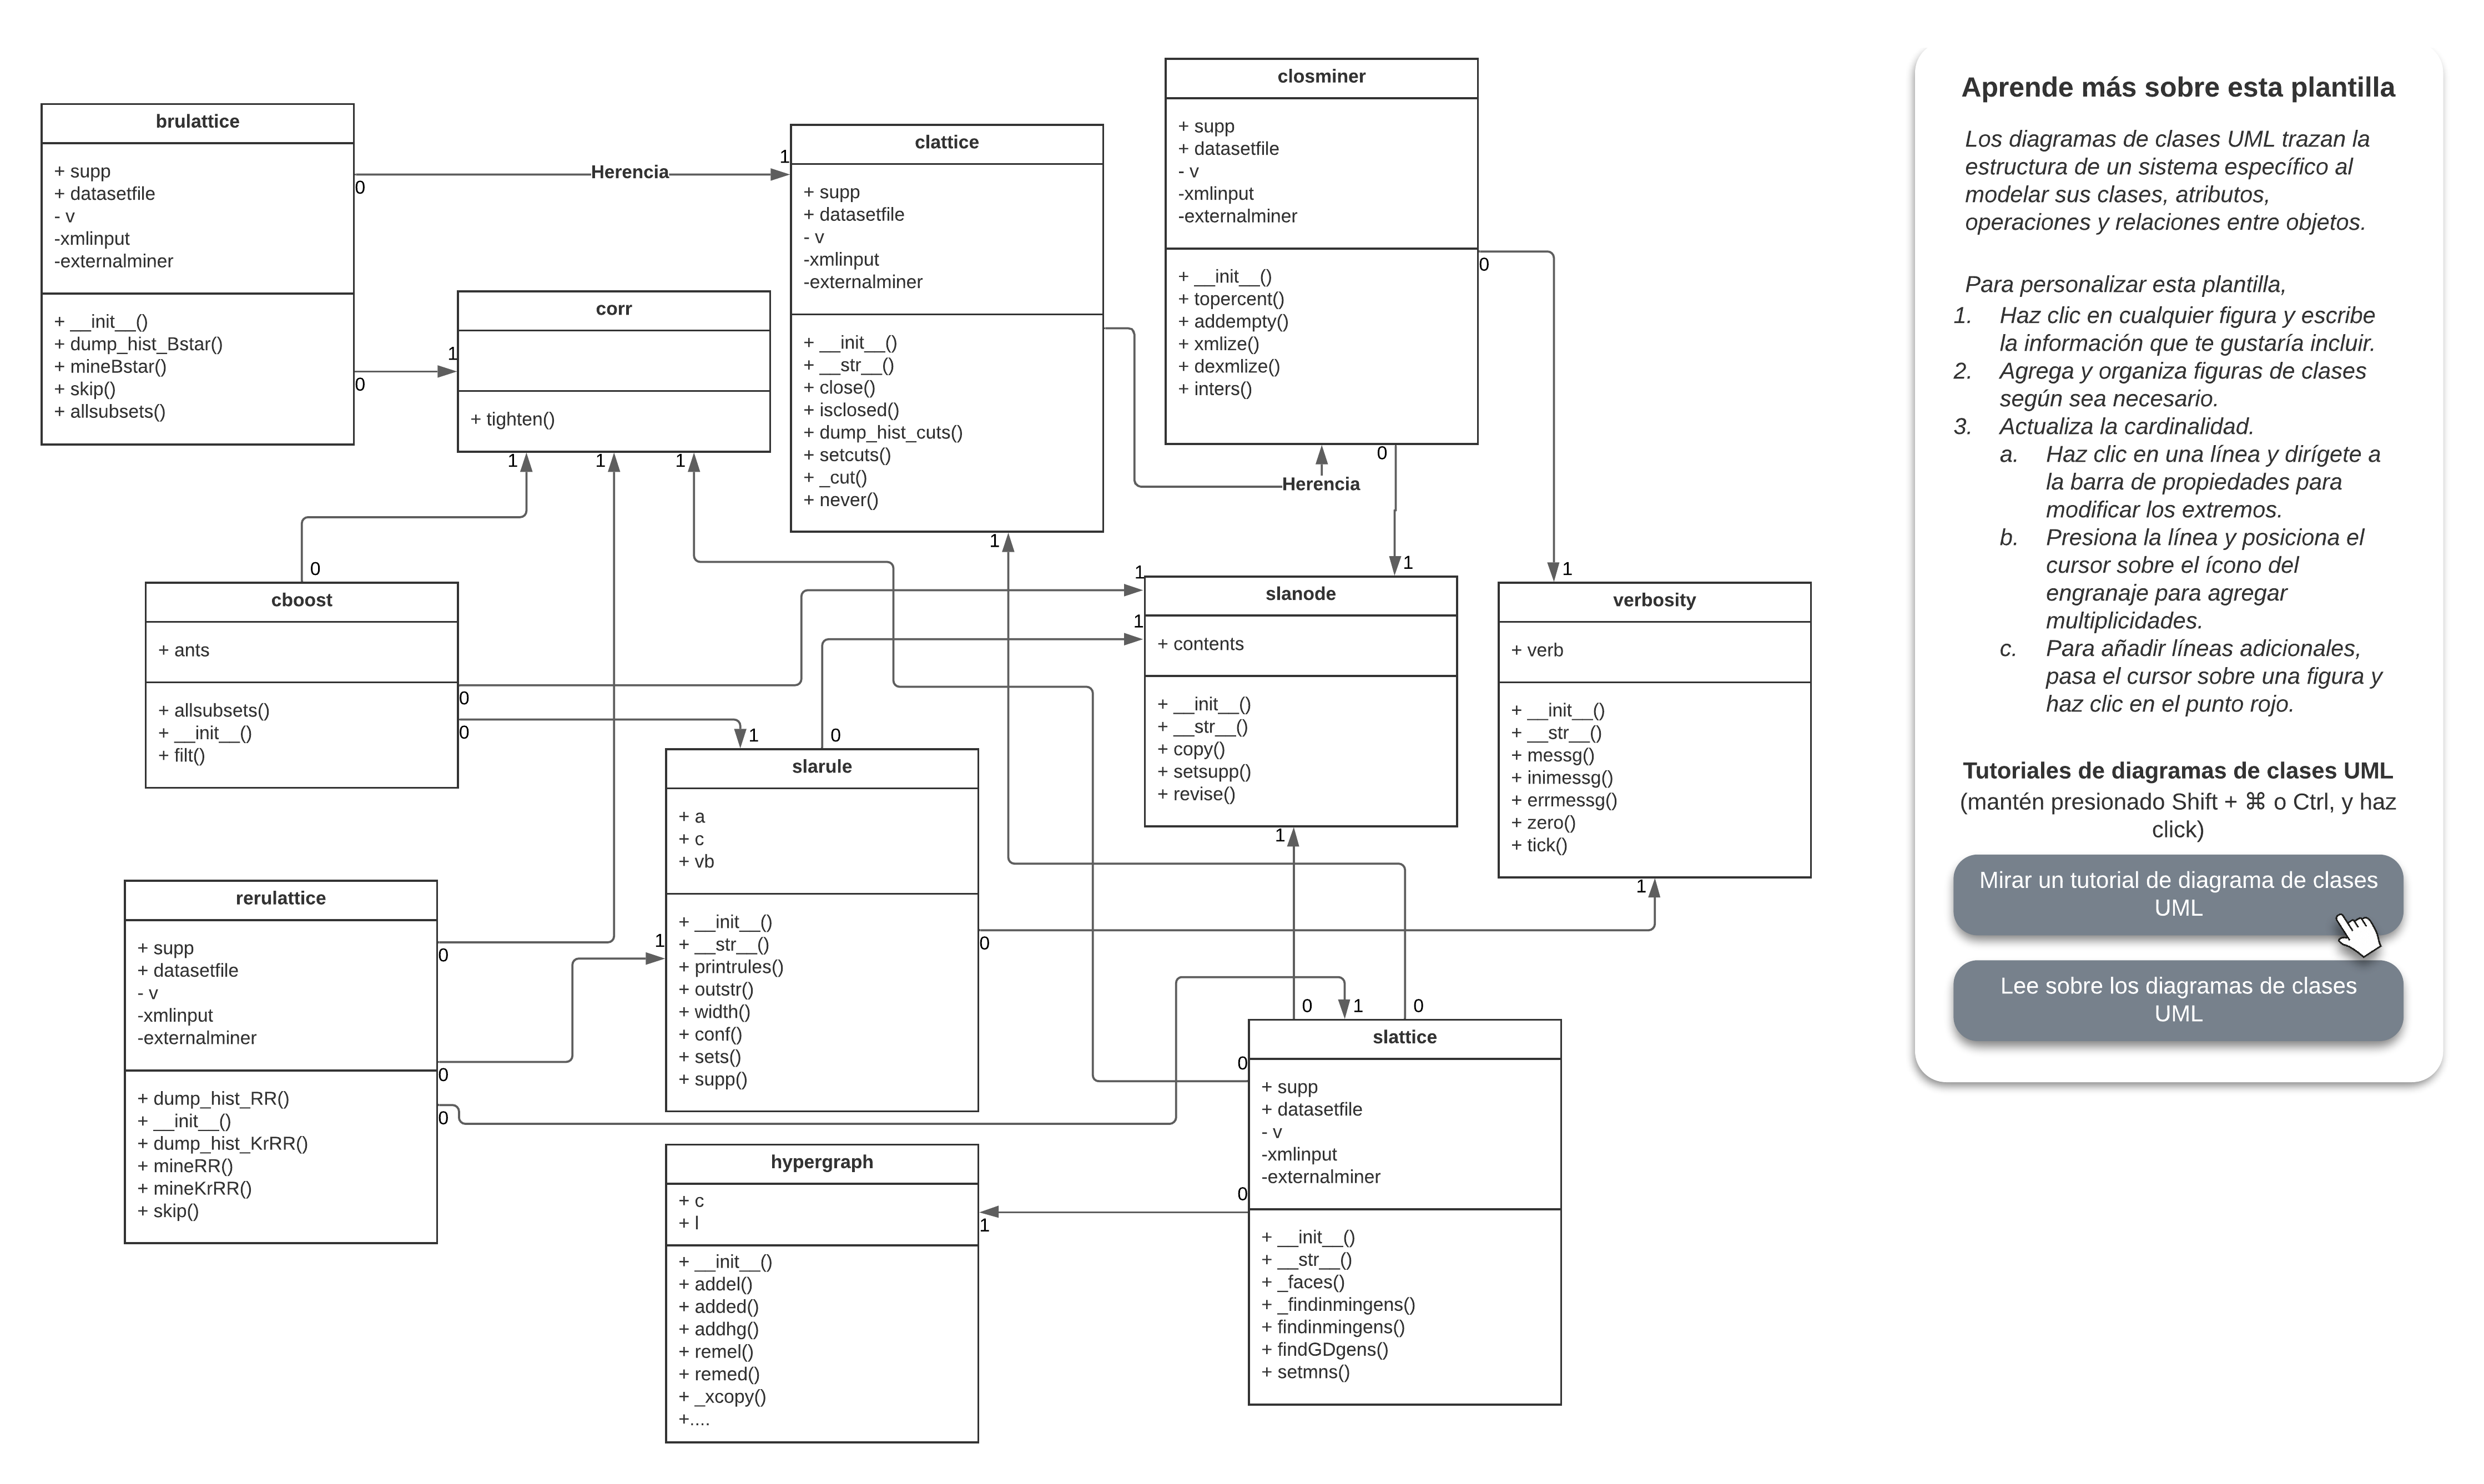
\includegraphics[width=1.5\linewidth]{imagenes/Diagrama en blanco - Clase UML (1).png}
\end{center}
\caption{Diagrama de clases UML Versión python2}
\label{fig_UML2}
\end{figure}

En este diagrama \ref{fig_UML2} se discutió sobre las conveniencias de cambiar este patrón, y se decidió no modificar el diagrama por diversas razones, uno de los motivos era que Slatt es era un aplicación muy estable y no se quería cambiar mucho la organización de sus clases, ya que sus usuarios que han aprendido a usar la versión antigua de Slatt no deberían volver a estudiarse el código, es por ello que solo se introdujo el patrón decorador en la clase decorator.py para añadir las funcionalidades de la metaprogramción al programa final. Como se puede comprobar en el la ilustración\ref{fig_UML3}.
\newpage

\begin{figure}[ht!] % [h!] fuerza que el elemento se sitúe
                    % en la posición señalada, en vez de al
                    % comienzo de una página.
\begin{center}
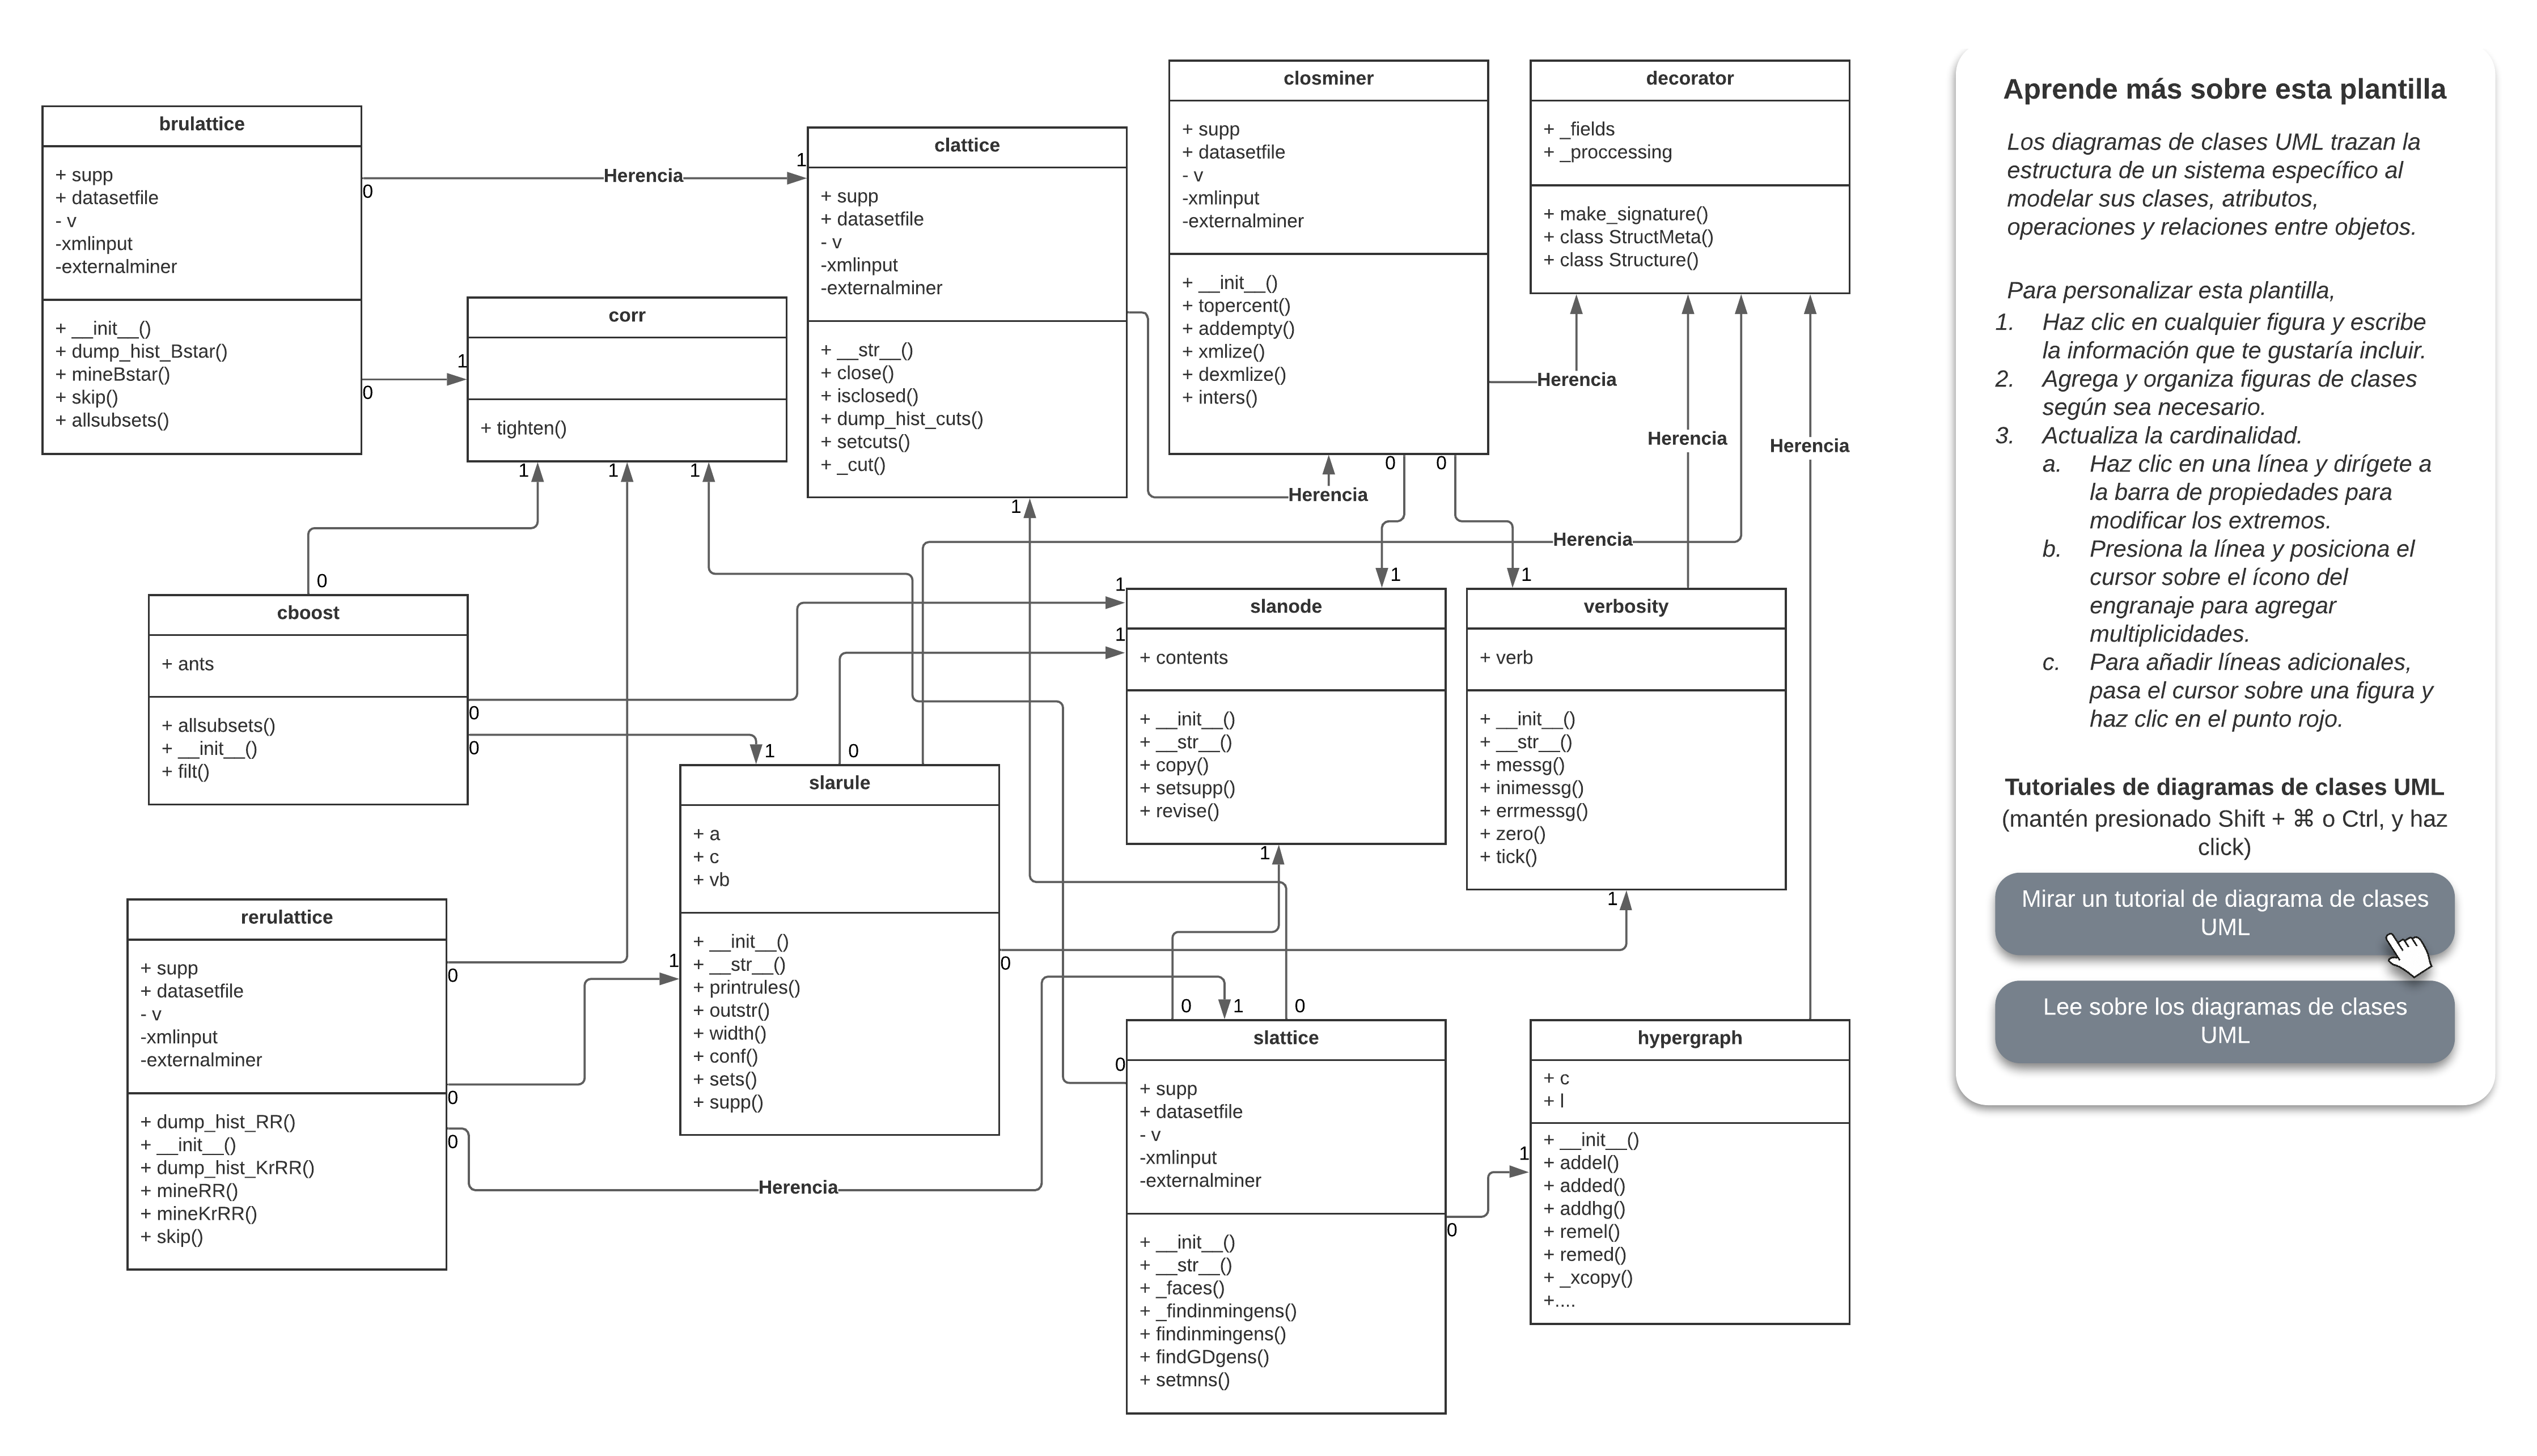
\includegraphics[width=1.42\linewidth]{imagenes/python3 - Clase UML.png}
\end{center}
\caption{Diagrama de clases UML Versión python3}
\label{fig_UML3}
\end{figure}

\newpage

\section{Diagrama de Gantt}

En esta otra sección indico como ha sido divido el proyecto en función del tiempo con un diagrama de Gantt \ref{fig_GANTT} en el que se ven las tareas que se han ido realizando durante el tiempo que el proyecto a estado activo.

\begin{figure}[ht!] % [h!] fuerza que el elemento se sitúe
                    % en la posición señalada, en vez de al
                    % comienzo de una página.
\begin{center}
\includegraphics[width=1\linewidth]{imagenes/Diagrama de Gantt básico.png}
\end{center}
\caption{Diagrama de clases UML Versión python3}
\label{fig_GANTT}
\end{figure}

Para implementar todos los requisitos no funcionales, después de cada reunión se decidió dividirlos en tareas, los requisitos \textit{RNF01, RNF03} se corresponden a la revisión del código ya que necesitábamos saber que partes del código se podían modificar y cuales no, para la reescritura de código se tuvieron en cuenta los requisitos \textit{RNF01, RNF02, RNF03, RNF04} ya que el código no debía de suponer ningún cambio en la funcionalidad del programa,  para los test unitarios y la corrección del código también se tuvieron en cuenta todos los requisitos no funcionales y en cuanto a la tareas de investigación (hipergrafos y kd-trees) se utilizó el \textit{RNF03} ya que se uso para hacer el código mas eficiente.



\chapter{\emph{Metaprogramación}}

\section{Introducción a la Metaprogramación}

Para satisfacer el RNF03 se decidió utilizar diferentes herramientas relacionadas con la metaprogramación en el entorno de desarrollo.

La metaprogramación consiste en escribir programas que manipulan otros programas, es decir, cuando un programa es capaz de recibir una entrada, modificar el contenido de dicha entrada durante su ejecución y producir como salida otro programa, es un metaprograma.

Una de las definiciones comúnmente aceptadas para metaprogramación seria "programar para generar código", esto ya existe desde Lisp. 
Esta propiedad se llama Homoiconicidad, es decir, es la propiedad de un lenguaje de programación por la que cualquier programa puede ser tratado como datos, ser manipulado y ejecutado.

No hay muchos lenguajes de programación que utilicen esta propiedad ya que implica una sobrecarga en memoria poder tener el programa en forma de datos, generalmente los lenguajes de programación que lo implementan son lenguajes funcionales, pero recientemente la versión de python 3.x decidió añadir tales funcionalidades. David Bleazley, unos de los desarrolladores oficiales de python, explica en esta charla uno de los grandes cambios que existen en python3 respecto de python2, la \textbf{metaprogramación}.\footnote{\citep{David}}

La parte principal de la charla es la utilización de los decoradores. La idea de los decoradores es definir funciones que definan nuevas funciones. La forma de implementarla se basa en la implementación que utiliza Lisp pero de una forma más rudimentaria. Se utiliza la nomenclatura decorador ya que no manipulan el código de la función, si no que definen una nueva función en base a la original, es decir, no la modifican pero se invoca.

En python3 se implementan estas ideas utilizando la clase \textit{decorators}, los \textit{descriptores} y las \textit{metaclases}.

\subsection{Usos de la Metaprogramación}

\begin{enumerate}
    \item Si queremos comprobar si una clase esta definida correctamente, podemos usar metaclases.
    \item Podemos usar metaclases para generar errores durante la importación de los módulos de la clase.
    \item Podemos usar la metaprogramación si queremos que nuestras clases tengan una convención especifica de métodos y atributos.
    \item Las metaclases se pueden utilizar para modificar el atributo de clase.
    \footnote{\citep{Farhad}}
\end{enumerate}

\newpage
\subsection{Conceptos teóricos básicos}
La metaprogramación se base en estos conceptos principales:

\begin{itemize}
    \item \textbf{Reflexión.- } La capacidad de un programa para observar y modificar su estructura.
    
    Un ejemplo de reflexión seria cuando el código fuente de un programa se compila, se suele perder información sobre la estructura del programa, pero si un sistema permite reflexión, se mantiene dicha estructura como metadatos en el programa generado.
    
    La reflexión se puede descomponer en dos partes:
    
    \begin{enumerate}
        \item \textbf{Introspección.- } La capacidad de un lenguaje de obtener información sobre si mismo.
        
        Un ejemplo de introspección seria java, en java se puede saber hasta nivel del método cuantos atributos, que tipos utiliza, etc.
        \item \textbf{Intercesión.- } La capacidad de modificar el propio comportamiento/ significado de la estructura del programa.
    \end{enumerate}
    
    \item \textbf{Reificación.- } La capacidad de convertir algo abstracto en un dato explícito.
    Ejemplos de reificación serian:
    \begin{itemize}
        \item Crear un tipo de satos para acceder a una posición de memoria
        \item Crear estructuras de datos que representan tipos abstractos de datos
    \end{itemize}
\end{itemize}

En conclusión la metaprogramación es la programación que utiliza los programas como datos y permite modificar su propia estructura. Aunque otra definición valida seria el conjunto de cosas que tienen más que ver con el proceso que con escribir código o trabajar de manera más eficiente\footnote{\citep{silva2018metaprogramacion}}.

\subsection{Elementos de metaprogramción en python3}
En general, las clases son la plantilla para la creación de objetos al igual que las \textbf{metaclases} son la plantilla de creación de las clases y por lo tanto, también son las plantilla para la creación de objetos.
La \textbf{Metainformación} son datos adicionales que aparecen en las clases y métodos de un programa. Como por ejemplo, de que tipo son las clases, el parámetro $\_\_doc\_\_$ ,que es la documentación relacionada a la clase, los métodos que tiene, atributos, etc. 

python3 utiliza una jerarquía para esta implementación, todo objeto pertenece a una clase menos las metaclases que están por encima de una clase, y no se pueden instanciar objetos de metaclases. La metaclases agrupan un conjunto de clases, y además podemos tener metainformación sobre clases dentro de una metaclase. 

\newpage

Por ejemplo:

\begin{verbatim}
def prueba_metaprogramacion():
class Prueba_met:
    pass
return Prueba_met

print(type(prueba_metaprogramacion))
print(type(prueba_metaprogramacion()))
\end{verbatim}

Este script escribe primero por la terminal \textit{<class 'function'>}, debido a que $prueba\_metaprogramacion$ es un objeto de la clase “function”. Mientras que en el segundo de los print la terminal devuelve: \textit{<class 'type'>}, debido a que el retorno de $prueba\_metaprogramacion()$ pertenece a la clase tipo.

La clase type es una metaclase. Esta clase se usa para crear otras clases en python. El constructor de dicha clase se usa para crear clases que pueden crear instancias de dicha clase.

\begin{verbatim}
##El constructor de la clase type tiene esta estructura

type(cls, what, bases=None, dict=None)
\end{verbatim}

El primer parámetro es el nombre de la clase, el segundo parámetro es una tupla de clases base, el tercer parámetro es un diccionario de llaves y valores, es decir, donde se debe implementar la clase.

Cuando creamos una metaclase que hereda la clase tipo, esta tiene acceso al nombre de la clase, sus padres y todos sus atributos.


\subsection{Clase Type}
El método estático $\_\_new\_\_$ se utiliza extensivamente en metaprogramación, ya que crea nuevas instancias de clase y no está vinculado a una instancia de la clase. Este método se invoca antes de llamar a $\_\_init\_\_()$. Podemos anular el $\_\_new\_\_()$ de la superclase.
El retorno del método $\_\_new\_\_()$ es la instancia de la clase. Esto es útil cuando queremos modificar la creación de tipos de datos inmutables como las tuplas.

En este proyecto utilizamos este tipo de funcionalidad en la clase decorator.py la cual tiene una clase llamada StructMeta la cual hereda de type e implementa el funcionamiento de el metodo $\_\_new\_\_()$.
\begin{verbatim}
class StructMeta(type):
def __new__(cls, name, bases, clsdict):
    clsobj = super().__new__(cls, name, bases, clsdict)
    sig = make_signature(clsobj._fields)
    setattr(clsobj, '__signature__', sig)
    return clsobj
\end{verbatim}



\subsection{Construir sistemas}
Otra funcionalidad que nos ofrece la metaprogramación es la construcción de sistemas, ya que para este tipo de proyectos, existe un "proceso de construcción", es decir, se necesita una secuencia de operaciones para transformar todas las entradas que metemos en salidas. Por lo general este proceso suele ser bastante tedioso ya que solemos tener una cantidad elevada de entradas, como por ejemplo, ejecuto un código para que funcione el programa, otro código para los benchmarks, otro código para los gráficos, es por ello que utilizamos la metaprogramación en este ámbito también.\footnote{\citep{metaprogramming}} Información sobre la construcción de sistemas.

Básicamente la funcionalidad es la siguiente, se define una serie de dependencias, una serie de objetivos y reglas para ir de uno a otro. Le indicas al sistema de compilación que objetivo desear ejecutar en particular, y el trabajo de este es buscar y encontrar todas las dependencias de ese objetivo, después aplicar las reglas que este contiene y llegar al objetivo final.

En este proyecto he usado uno de los sistemas de compilación más conocidos en el ámbito de la programación \textbf{make}, debido a que el proyecto a sido totalmente desarrollado en linux y make esta instalado en cualquier maquina que utilice UNIX como sistema operativo. En este caso he usado dicho sistema para generar la memoria en latex y para la ejecución de los test unitarios y benchmarks, un ejemplo de ello son los siguientes objetivos marcados:

\begin{verbatim}
    paper.pdf: paper.tex plot-data.png
	    pdflatex paper.tex
\end{verbatim}

La directiva paper.pdf tiene una regla sobre cómo producir el lado izquierdo usando el lado derecho. O, dicho de otra manera, las cosas nombradas en el lado derecho son dependencias y el lado izquierdo es el objetivo. En make, la primera directiva también define el objetivo predeterminado. Si ejecuta makes sin argumentos, este es el objetivo que construirá.



\chapter{\emph{Hipergrafo y problemas relacionados}}

\section{Conceptos teóricos básicos}
En dicho proyecto también se van a tratar elementos como los hipergrafos
y algoritmos con aplicación a estos, para ello primero se ha realizado un primer apartado con los conceptos básicos sobre los hipergrafo y más adelante introduzco una explicación más técnica y profunda en el tema.

Un hipergrafo H es una familia de subconjuntos (aristas) de un conjunto finito de vértices. Un hipergrafo es simple si ninguno de sus aristas está contenido en ningún otro de sus aristas. Decimos que un hipergrafo está saturado si cada subconjunto del conjunto de vértices está contenido en una arista o contiene una arista de el hipergrafo. \citep{Thomas}

Se toma como algoritmo principal \textit{The algorithm of Berge}, al cual se le añadirán diferentes mejoras analizadas y comprobadas en el paper desarrollado por \citep{JGAA-107} el cual implementa un algoritmo eficiente para la generación "transversals" de hipergrafos.


% Añadiendo la opción «commandchars=\\\{\}», los caracteres
% \, { y } del archivo fuente se interpretan como código
% LaTeX y puede darse formato al código (manualmente). Hay
% que tener esto en cuenta cuando estos caracteres formen
% parte del código en sí.
%
% Sin esa opción, el fichero de reproduce tal cual.

\begin{center}
% Puede pasar parámetros al comando «VerbatimInput» del
% paquete «fancyvrb». Por ejemplo:


\lstinputlisting[language=python,caption=\textbf{Original Berge Algorithm},frame=bottom]{codigo/berge.py}

\lstinputlisting[language=python,caption=\textbf{Efficient Berge Algorithm},frame=bottom]{codigo/bergeMod.py}


%\codigo[numbers=none,frame=single]{codigo/berge.c}{Original}{11.5cm}

\end{center}
\newpage
\section{Problemas relacionados con SIMPLE-H-SAT en la teoría de bases de datos}

Uno de los principales problemas de los hipergrafos es el conocido como SIMPLE HYPERGRAPH SATURATION o SIMPLE-H-SAT, el ejemplo más utilizado para su explicación y que además aparece en el artículo \citet{Thomas} es el problema de "La pizzería de Toni".

Toni tiene un hermano llamado Luigi, que también tiene una gran pizzería. Luigi está orgulloso de que cada una de sus pizzas es 'original', lo que significa que en su restaurante no hay versiones de pizzas Grande o Mini. Como se entera de los planes de su hermano, Luigi también tiene la intención de ampliar su oferta de pizza por una pizza nueva, que, por supuesto, tiene que ser una pizza 'original'. Está claro que el problema de Luigi es una versión restringida del problema de Toni. Dado que todas las pizzas son 'originales', en el correspondiente problema de saturación del hipergrafo, el hipergrafo de pizza es simple. Pero la verdadera cuestión que plantea este problema, es si la restricción en la entrada hace que el problema general de saturación sea manejable, con un numero de entradas mayor no únicamente dos entrada como en este caso.

\begin{figure}[ht!] % [h!] fuerza que el elemento se sitúe
                    % en la posición señalada, en vez de al
                    % comienzo de una página.
\begin{center}
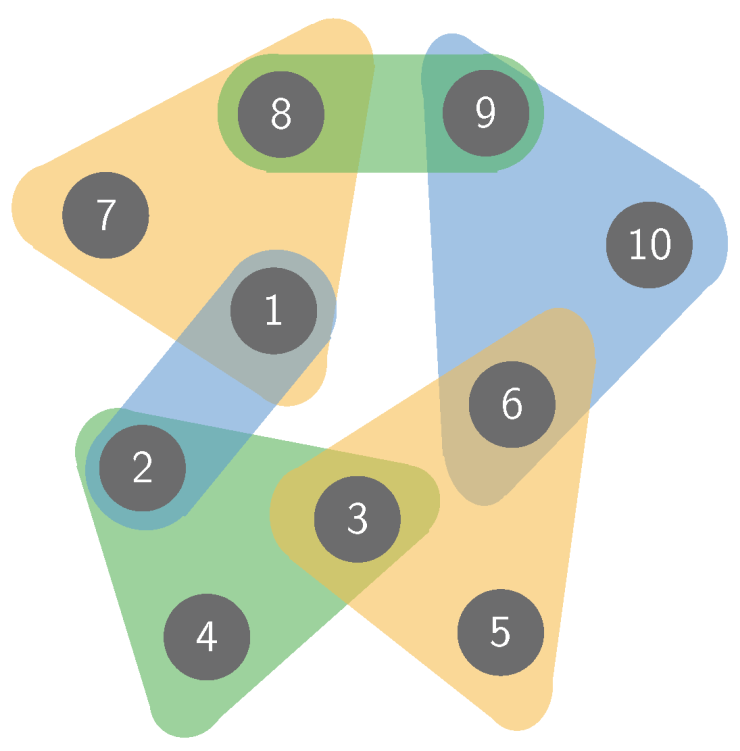
\includegraphics[width=0.4\linewidth]{imagenes/S-H-SAT.png}
\end{center}
\caption{Ejemplo gráfico del SIMPLE-H-SAT}
\label{SHSAT}
\end{figure}

Siguiendo la lectura del artículo en el apartado séptimo habla sobre las bases de datos relaciones y hace una explicación sobre como esta formada una relación, básicamente una una relación es una tabla de tuplas distintas de pares de componente que son valores de los dominios de los atributos. Por ejemplo, $U = \{A_0,A_1,...,A_n\}$ es un conjunto de atributos, cada uno de los cuales está asociado a un dominio D. Entonces $D(A_i)$ es el dominio de un atributo $A_i$. 
Entonces una relación sobre U es un subconjunto de $\prod_{i=1}^{n}D(A_i)$, y el los elementos de una relación se denominan tuplas.

El artículo también habla sobre las relaciones funcionales, es decir, esas reglas de asociación que nos dan una información de unas variables frente a otras, y lo explica de la siguiente manera:

"Dados los conjuntos $ X, Y $ de atributos, la dependencia funcional (FD) $ X \rightarrow Y $ se mantiene en la relación R si en cada tupla los valores de los atributos en Y están determinados únicamente por los valores de los atributos en X, para tuplas $ t_1 , t_2 \in R \;; t_1 [X] = t_2 [X] $ implica que $ t_1 [Y] = t_2 [Y]: $ Dado que posiblemente todas las tuplas de una relación tienen los mismos valores para algún atributo, el lado izquierdo X de un FD $ X \rightarrow Y $ puede estar vacío. Si $Y \subseteq X$, entonces se llama dependencia funcional trivial."

\newpage

Y en general, explica como conseguir relaciones funcionales válidas, para ello se tienen que definir diferentes términos.

\begin{itemize}
    \item \textbf{Conjuntos cerrados.-} Son los que no puedes ampliar sin perder soporte. Formalmente hablando, un conjunto $X \subseteq I$ es cerrado si $X=X$, donde $X$ es la clausura de $X$ y se calcula con la $formula :X=\{a \in I |s( X \cup\{a\}) = s(X)\}$
    
    \item \textbf{conjuntos frecuentes.-} $F_\tau=\{X \subseteq I \;|\; s(X) \geq \tau\}$
    \item \textbf{conjuntos frecuentes cerrados.-} $FC_\tau=\{X \in F_\tau \;|\; \forall Z \supset X,s(Z)<s(X)\}$
    \item \textbf{generadores minimales frecuentes.-} $\{X \in F_\tau \;|\; \forall Y \subset X,s(Y)>s(X)\}$
    
\end{itemize}

Con estos elementos definimos si una regla es redundante, sirve para no llenar la base de datos de una misma regla de asociación que se repite durante el tiempo, ocupa espacio innecesario y no ofrece ningún tipo de información valiosa.

Después de la definición de los anteriores conceptos, podemos decir  que una regla de asociación es:

$AR_\tau,_\gamma=\{X\rightarrow Y \;|\; s(X \rightarrow Y)\geq \tau,c(X \rightarrow Y) \geq \gamma\}$, siendo $\tau$ y $\gamma$ umbrales de soporte y confianza respectivamente.

También podemos definir la reglas representativas como:

$RR_\tau,_\gamma=\{r \in AR_\tau,_\gamma \;|\; \nexists \; r′ \in AR_\tau, \;|\; \gamma\{r\}$ tal que $r \in C(r′)\}$ \citep{UC}

Con esta definición de regla representativa no redundante podemos conseguir una cantidad de reglas de asociación menor con un mismo valor de contenido, es decir, nos ahorraríamos mucho espacio en una base de datos gracias a esta definición de regla representativa.


\section{Problemas relacionados con 'Hypergraph Transversals' y su saturación}

El segundo problema que nos encontramos después del SIMPLE-H-SAT es el reconocimiento de las 'transversals' mínimas de un hipergrafo, ahora indicaré cual es la complejidad de dicho problema y luego demostrare la equivalencia que tiene con SIMPLE-H-SAT y el reconocimiento transversal en tiempo polinomial, basándome en la definiciones del artículo anteriormente mencionado \citep{Thomas}.


\textbf{Definición 1.} Teniendo dos hipergrafos \textit{H}, \textit{G} con vértices \textit{V}. Entonces $H \geq G$ si y solo si $\forall h \in H : \exists g \in G : H \supseteq G$. Esto a su vez define la siguiente relación,  $H \leq G$ si y solo si $\forall h \in H : \exists g \in G : H \subseteq G$.

Decir que  \textit{H} = \textit{G} si y solo si $H \geq G$ y $G \geq H$, y $H \geq G$ no implica que $G \leq H$ y viceversa. Ahora indico una caracterización para la saturación de los hipergrafos:

\textbf{Teorema 1.} $H \neq \emptyset$ puede ser un hipergrafo. Entonces H esta saturado si y solo si $Tr(max(H)) \geq min(H)$.

\textbf{Prueba:} Asumimos que \textit{H} esta saturado, y consideramos una arista \textit{T} de $Tr(max(H))$. Tenemos $T \in Cov(H)$, pero T es una transversal de $max(H)$, $\forall E \in H $ se mantiene que $T \nsubseteq E$. Pero entonces $E' \subseteq T$ para algún $E' \in H$ lo que implica que $T \supseteq E''$ para algún $E'' \in min(H)$. Esto implica que $Tr(max(H)) \geq min(H)$. Asumimos ahora que \textit{H} no esta saturado, $X \supseteq V, X \notin Cov(H)$.

\textbf{Corolario 1.} Un hipergrafo $H \neq \emptyset$ es saturado si y solo si $Tr(\overline{H}) \geq H$.

\textbf{Prueba:} Es fácilmente demostrable que $\overline{max(H)} = min(\overline{H})$, sacado directamente del Teorema 1

\textbf{Corolario 2.} Para demostrar si $Tr(H) \geq H$ se sostiene para un hipergrafo H es co-\textbf{NP}-completo, incluso si \textit{H} se auto completa y contiene solo aristas de tamaño 3 y n-3, donde $n = |V(H)|$

\newpage

\section{Axiomas de Armstrong}

Los Axiomas de Armstrong son en su esencia reglas de inferencia mencionadas anteriormente.
Estas reglas permiten deducir todas las dependencias funcionales que tienen
lugar entre un conjunto dado de atributos $A=\{A_1,A_2,...,A_n\}$ , como consecuencia de las dependencias dadas, es decir, se deducen todas las dependencias que se asumen ciertas a partir del conocimiento del problema.

\subsection{Ejemplo de axiomas de Armstrong}
Tenemos una relación R con tres atributos (A,B,C), ahora, después de realizar la función de dependencias, nos devuelve las dos siguientes reglas $F = \{A \rightarrow B , \; B \rightarrow C\}$, con estas dos reglas podemos inferir el conjunto completo de funciones de dependencias que serian: $\{ A \rightarrow C , A \rightarrow A , B \rightarrow B , C \rightarrow C ,\}$.

Ahora tenemos un set F con las dos reglas de dependencias y un superset $F^+$ el cual es un set de funciones lógicamente inferidas de F. A continuación, muestro una tabla de la relación entre el numero de atributos combinados y las posibles keys que podemos elegir.

\begin{table}[h]
\begin{tabular}{|l|l|l|l|}
\hline
                               & \multicolumn{3}{l|}{\# de atributos combinados} \\ \hline
\multirow{4}{*}{Posibles keys} & 1              & 2               & 3                \\ \cline{2-4} 
                               & A              & AB              & ABC              \\ \cline{2-4} 
                               & B              & AC              &                  \\ \cline{2-4} 
                               & C              & BC              &                  \\ \hline
Total                          & 3              & 3               & 1                \\ \hline
\end{tabular}
\end{table}

En este caso es sencillo debido a que únicamente tenemos 3 atributos posibles, pero en el caso que por ejemplo tengamos un numero elevado de ellos A = 100 se puede utilizar una formula matemática que calcula el numero de posibilidades $\frac{n!}{(n-r)! (r)!}$ donde r es número total de atributos y n cuantos atributos por key tenemos.

Una vez tenemos esto necesitamos un mecanismo que nos permita conocer si las reglas de dependencia están dentro o fuera del $F^+$, es entonces cuando utilizamos los axiomas de Armstrong.

Para ello primero definiré que es un axioma, según la tercera definición del diccionario, un axioma es una proposición que se asume sin prueba, con el fin de estudiar las consecuencias que se derivan de ella. Los axiomas de armstrong tienen tres acciones reflexividad, aumentatividad y transitividad, que son en términos matemáticos definidas de la siguiente manera:

\begin{enumerate}
    \item \textbf{Reflexividad} $\forall X , X \rightarrow X $ $ex. (ABC \rightarrow AB)$
    
    \item \textbf{Aumentatividad} $\{ X \rightarrow Y , Z \supseteq X \} \Rightarrow Z \rightarrow Y  $ $ex. (AC \rightarrow CB)$
    
    \item \textbf{Transitividad} $ \{ X\rightarrow Z , Z \rightarrow Y \} \Rightarrow X \rightarrow Y $ $ex. (A \rightarrow B , B \rightarrow C) \Rightarrow (A \rightarrow C)$
\end{enumerate}

Si tenemos en $F^+$ un set de todas las funciones con dependencias las cuales hemos inferido de F, si aplicamos las acciones de armstrong a F no vamos a encontrar ningún set de funciones con dependencias fuera de F solo podremos encontrar estas funciones dentro de F.

Otro aspecto de los axiomas de armstrong es que es completo esto quiere decir que si aplicamos acciones de armstrong a F vamos a encontrar todas las funciones con dependencias existentes en dicho set.




\chapter{\emph{KD Trees}}

\section{Introducción a los KD-trees y usos}
Una de las operaciones que hemos detectado que más se repiten en la ejecución del código es comprobar que items contienen cierto numero de transacciones. KD-trees es una estructura de datos cuyo objetivo es mejorar la complejidad computacional mediante un preproceso de los datos.

Los kd-trees son frecuentemente utilizados en bases de datos para satisfacer consultas que incluyan valores de varios campos. Esto se puede extrapolar a las reglas de asociación, ya que se podrían realizar consultas como se ha explicado en el ejemplo introductorio de reglas de asociación.

\hspace{0.5mm}

Una consulta podría ser por ejemplo, saber todos los registros de personas que compren pan, leche y huevos, y además tengan entre 25 y 45 años, y que vivan en España, todo esto se podría realizar en una única consulta utilizando los \textit{KD trees} como algoritmo de búsqueda ya que permite realizar diferentes consultas simultaneas, en lugar del algoritmo \textit{apriori} actualmente utilizado, en el que al añadir múltiples consultas, su coste computacional hace que no tenga sentido dicho calculo, debido a su lento proceso.

\section{Conceptos básicos}

Un KD Tree (también conocido como K-Dimensional Tree) es un árbol de búsqueda binario donde los datos en cada nodo son un punto k-dimensional en el espacio. Básicamente, es una estructura de datos que utiliza una partición en el espacio para organizar puntos en un espacio K-Dimensional.

\begin{enumerate}
    \item Cada nodo tiene como clave multidimensional un vector de tamaño k
que contiene los valores de las k claves unidimensionales y tiene asociado un discriminante \footnote{El discriminante es un nuevo elemento que se introduce en los kd-trees para manejar elementos con claves de más de una dimensión} con valor entero entre 1 y k.
    \item Para cada nodo con clave multidimensional x y discriminante j se
cumple que cualquier nodo del subárbol izquierdo con clave multidimensional y cumple que su n-ésima componente es menor que la n-ésima componente de x, es decir (yn < xn ). Para el subárbol derecho se cumple que la n-ésima componente de la clave multidimensional z de cualquier nodo de este subárbol es mayor que la n-ésima componente de la clave x, es decir (zn > xn ).
    \item La raíz del kd-tree tiene profundidad 0 y discriminante 1. Cualquier
nodo a una profundidad p tiene discriminante de valor: (p mod k) + 1.
\citet{bentley1975multidimensional}
\end{enumerate}

Otra de las aplicaciones es la de representar un conjunto de puntos y la consulta más frecuente sobre este conjunto es la de localizar el punto o puntos más cercanos a uno dado. Esta consulta se conoce con el nombre de búsqueda del vecino más cercano.

\newpage

\section{Ejemplo gráfico KD Tree}

\hfill

Ejemplo gráfico de un KD-tree para el siguiente ItemSet:

\textbf{{(3,6),(17,15),(13,15),(6,12),(9,1),(2,7),(10,19)}}

\hfill

\begin{figure}[h]
\begin{center}
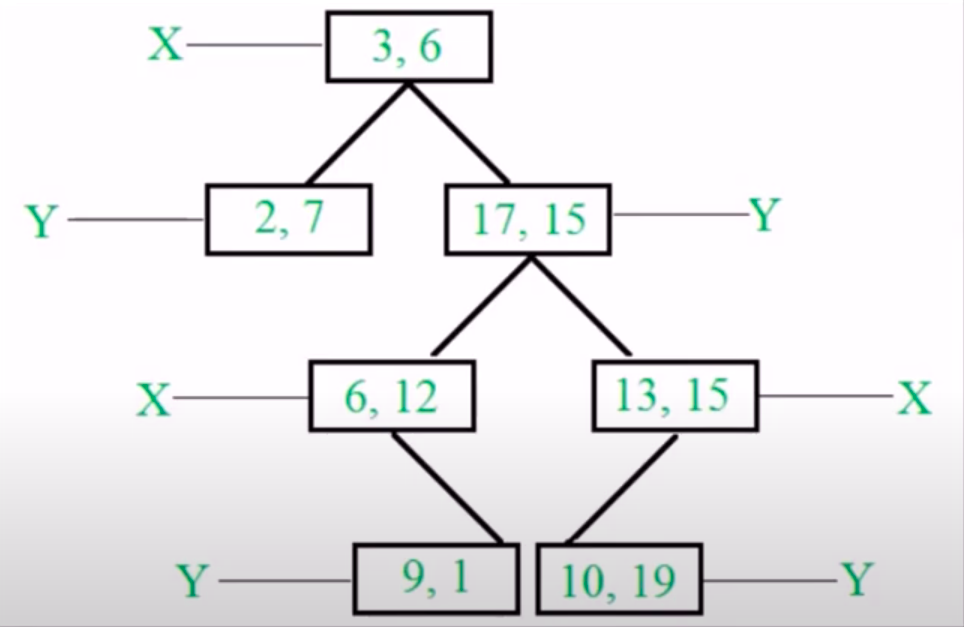
\includegraphics[width=.4\linewidth]{imagenes/kdtree1.png}
\end{center}
\caption{Árbol del ItemSet}
\label{arbol_kd}
\end{figure}

\begin{figure}[h]
\begin{center}
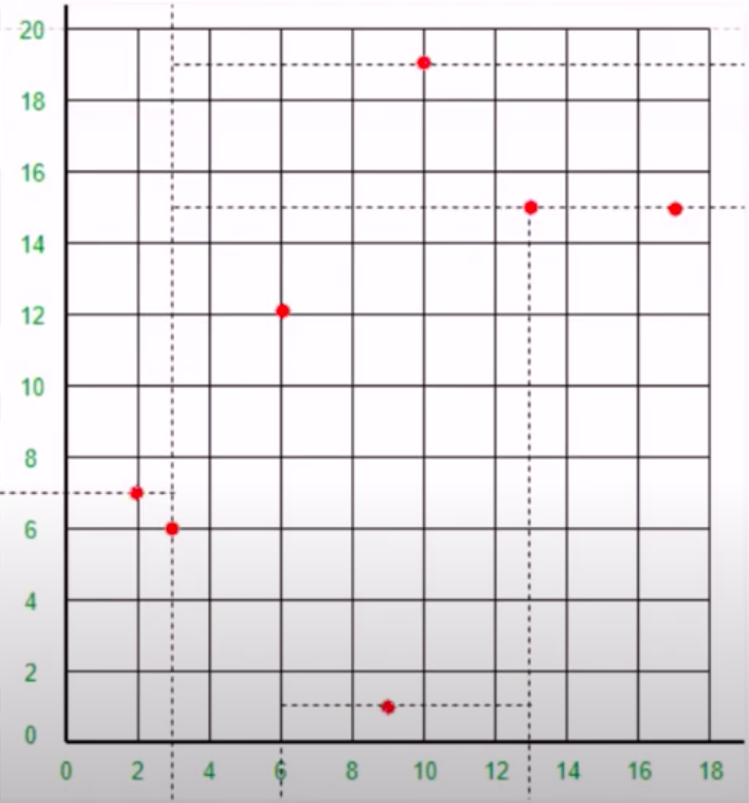
\includegraphics[width=.4\linewidth]{imagenes/kdtree2.png}
\end{center}
\caption{Gráfica del ItemSet}
\label{grafica_kd}
\end{figure}

Desde un punto de vista geométrico como se ve en la Ilustración \ref{arbol_kd}, cada nodo del kd tree hace una partición del plano en dos “subplanos”. En la Ilustración \ref{grafica_kd} todos los puntos en el “subplano” de la izquierda corresponden al subárbol izquierdo del nodo raíz, y los que quedan a la derecha son los puntos del subárbol derecho.


\section{Implementación KD-Trees en Slatt}

Se acordó en la reunión de la semana 3 que no era óptimo usar la implementación realizada con kd-trees debido a que para una cantidad menor de n datos los resultados que obtuve no mejoraban e incluso empeoraban el rendimiento de Slatt, esto es debido, a que usando este tipo de estructura de datos, se necesita una carga de datos elevada en memoria para poder exprimir al máximo el poder computacional que tiene, si usamos pocos datos como era el caso, además usando este tipo de estructura de datos no se satisfacía el requisito no funcional \textit{RNF02}, por lo que la descartamos, y nos quedamos con la explicación meramente teórica de los kd-trees, que nos podría servir para un problema más grande que el que se trata en este proyecto.


\chapter{\emph{Desarrollo Software}}
En este aparatado del proyecto se muestran que cambios han sido necesarios en el código para la correcta ejecución de Slatt pasando todo su código de python2 a python3, los test necesarios para su correcto funcionamiento y además se explica que mejoras se han llevado a cabo tanto de rendimiento, como en la reducción del número de lineas de código.

\section{Ejecución y funcionamiento de Slatt}

Slatt es una herramienta matemática que se encarga de mediante una entrada de datos en este caso, por ejemplo, un dataset sobre los problemas de visión de ciertas personas, el cual dispone de 4 atributos, la edad, la prescripción (myope, hypermetrope,etc), si tiene o no astigmatismo y la cantidad de lágrimas que genera.

Se introduce dicho dataset en el programa principal y la herramienta devuelve diferentes datos como son la confianza, el soporte y con esto generar las diferentes reglas de asociación que existen y cuales de estas son reglas de inferencia. 

\section{Test unitarios}

En esta sección se especifica como se realizan los test unitarios, para comprobar si las dos versiones del código mantienen la misma funcionalidad basándose en la salida de estos test.

\hfill

\lstinputlisting[language=bash,caption=\textbf{Makefile},frame=bottom]{codigo/makefile}

Utilizando este \textbf{makefile} se realiza una ejecución simultanea de ambas versiones, guardando dicha salida en un fichero.txt y a continuación, se hace un \textbf{diff} entre los dos archivos, en el caso en el que el \textbf{diff} devuelva un archivo vacío, sabremos que las dos versiones tienen la misma funcionalidad.

\newpage

\section{Mejoras del código}
En esta sección se va a discutir cuales han sido los cambios y mejoras en cada una de las clases que se han modificado en el código:

\subsection{Diferencias entre python2 y python3}

En la actualidad, existen dos tipos de versiones de python, las cuales son 2.x en la que está inicialmente escrita Slatt y 3.x en la cual se ha estado desarrollado este proyecto.

Las principales diferencias que he encontrado en el proyecto han sido las siguientes \citet{diferencias}:

\begin{enumerate}
    \item \textbf{Sentencia print}
    
    Esta posiblemente sea la diferencia que más veces ha aparecido en el proyecto, ya que en prácticamente todas y cada una de las clases aparece algún print en el main o en algún método de la propia clase.
    Se soluciona de una manera muy sencilla, añadiendo el el argumento de la sentencia print dos paréntesis. (print \textbf{x} --> print( \textbf{x} ))
    
    \item \textbf{Comparación de tipos}
    
    En \textbf{python2} se permiten las comparaciones entre objetos de distintos tipos, mientras que en \textbf{python3} nos lanza una excepción del tipo \textit{TypeError}, esto a sido necesario tenerlo en cuanta en el código porque había bastantes comparaciones de tipos distintos a lo largo del código en clase como brulattice.py o closminer.py.
    
    \item \textbf{División de números enteros}
    
    En \textbf{python2} la división entre números enteros da un numero entero y si quieres conseguir un resultado con decimales necesitas que uno de los dos números de la operación tengan un decimal, en este caso en \textbf{python3} se hace mediante un truncado de la división usando el // en lugar de /.
    
    \item \textbf{Iterar un diccionario}
    
    Otra diferencia que se ha detectado en código a la hora de hacer la reescritura a \textbf{python3} a sido la iteración de diccionarios ya que en \textbf{python2} se pueden iterar los elementos clave-valor de un diccionario con el método \textit{iteritems()} o \textit{items()}, mientras que en python3 únicamente se puede usar el segundo de estos dos métodos, ya que con el primero de ellos se produce una excepción de tipo \textit{AttributeError}.
    A su vez, los métodos \textit{iterkeys()} e \textit{itervalues()} para iterar las claves y los valores de un diccionario respectivamente no existen en python 3. En su lugar tenemos que usar los métodos \textit{keys()} y \textit{values()}. Estos métodos tanto \textit{keys()}, \textit{values()} como items() se han visto afectados en clases como brulattice.py o cboost.py
    
    \item \textbf{Patrón decorador}
    
    Por ultimo, una de las grandes y más importantes diferencias que se ha encontrado es la metaprogramación, en concreto el patrón decorador, esta funcionalidad ha sido utilizada en la versión de python3, ya que nos ofrece una reducción de código a la hora de definir funciones que se repiten en una misma clase.
    
\end{enumerate}
\newpage
\subsection{Cambios realizados en las clases}

\begin{itemize}

\item \textbf{brulattice.py}

En la clase brulattice.py no se han realizado mejoras ni cambios en el código salvo lo necesario para la ejecución en python3. (\# lineas antes = 93, \# lineas después = 93)

\item \textbf{cboost.py}

En la clase cboost.py inicialmente he modificado el método allsubsets para que sea mas corto y eficiente utilizando la librería de combinations procedente de itertools la cual me permite realizar fors anidados de una manera más eficiente y con un número de lineas reducido. (\# lineas antes = 45, \# lineas después = 40)

\begin{verbatim}
    def allsubsets(givenset):
    aset = givenset.copy()
    for e in aset:
        aset.remove(e)
        p = allsubsets(aset)
        q = []
        for st in p:
            s = st.copy()
            s.add(e)
            q.append(s)
        return p+q
    return [ set([]) ]
    
    #### Se sustituye por: #####
    
    def allsubsets(givenset):
    s = len(givenset)
    q=[]
    for i in range(s):
        for e in combinations(givenset,i):
            q.append(e)
    return q
\end{verbatim}

Dentro del método \textit{filt()} también se han cambiado alguno de los fors anidados que tenia debido a que aumentaban la carga de trabajo innecesariamente, para ello en vez de utilizar el método \textit{keys()} a la hora de iterar, se ha decidido utilizar dos parámetros en el for e iterarlo sobre el método \textit{items()}, con lo que mejoramos tanto la legibilidad del código como el rendimiento ya que nos eliminamos un for anidado por cada vez que lo sustituimos, el único inconveniente encontrado en este paso fue que al usar este tipo de for no puede haber dependencias entre ambos parámetros ya que entonces no funciona correctamente el programa. (\# lineas antes = 60, \# lineas después = 52)

\begin{verbatim}
    for cn2 in rrseconf.keys():
        for an2 in rrseconf[cn2]:
        
     #### Se sustituye por: #####
     
     for cn2,values in rrseconf.items():
        for an2 in values:
\end{verbatim}

\item \textbf{clattice.py}

En la clase clattice.py utilice la variable \_processing para eliminar el \_\_init\_\_ el cual era muy largo y costoso definiéndolo en un método fuera de la clase el cual se ejecuta una vez y no es necesario volver a ejecutar con lo que a la larga nos ahorramos código en tiempo de ejecución, por lo demás no he incluido ninguna mejora más respecto a python2. (\# lineas antes = 154, \# lineas después = 136)

\item \textbf{closminer.py}

En la clase closminer.py se ha realizado un cambio similar al de clattice.py introduciendo una método pos\_init que funciona como método auxiliar para la creación de una instancia de closminer, además de introducir la herencia de la clase structure de decorator para poder eliminar el método \_\_init\_\_ y así acelerar el proceso como hemos hecho en las demás clases del programa. (\# lineas antes = 300, \# lineas después = 84)

\item \textbf{corr.py}

La clase corr.py es una clase con pocas lineas de código y difícil de optimizar más ya que no contiene método muy densos, por que únicamente he realiza la herencia de Structure y he eliminado el constructor ineficiente que teníamos en python2. (\# lineas antes = 49, \# lineas después = 22)

\item \textbf{decorator.py}

La clase decorator.py es una nueva clase implementada para \textbf{python3} la cual nos permite utilizar diferentes funcionalidades de la metaprogramación mencionadas anteriormente, como es la creación de constructores mediante una simple linea de código gracias a las clase Structure  y la variable \_fields o incluso introducir partes del código (funciones, métodos) con otra variable llamada \_processing.

También se introducen un método que nos permite saber quienes son las clases padre de una clase u objeto, gracias al modulo \textit{Signature} de la clase inspect.py. (\# lineas antes = 0, \# lineas después = 72, se añaden lineas debido a que es una clase nueva)

\item \textbf{hypergraph.py}

En la clase hypergraph se realiza una herencia de la clase Structure, para eliminar su \_\_init\_\_ sustituyéndolo por la variable \_fields y con ello reducir el número de lineas de código.
También se ha diseñado un patrón decorator el cual sustituye la mayoría de las funciones que se encuentran en dicha clase:  \textbf{[addel,added,addhg,remel,remed]}, este cambio se llevó a cabo debido a que se vio un claro patrón de repetición en todas las funciones de la clase, el patrón es el siguiente:

\begin{verbatim}
        def decorator(self,a1,a2,a3,a4,a5):
        if a1:
            a1()
        for e in a2:
            a3(e)
        if a4:
            a4(a2)
        if a5:
            a5()
\end{verbatim}

Con este patrón se consigue resumir todas y cada una de las funciones de la clase en una única linea de código, para ello tuve que usar funcionalidades como \textit{lambda} la cual permite generar una función dentro del patrón decorator. (\# lineas antes = 142, \# lineas después = 134)

\item \textbf{rerulattice.py}

En la clase rerulattice.py no se han realizado mejoras ni cambios en el código salvo lo necesario para la ejecución en python3. (\# lineas antes = 101, \# lineas después = 101)

\item \textbf{slanode.py}

En esta clase slanode.py se ha eliminado la clase \textit{auxitset} con todos sus métodos, introduciéndola dentro de la propia clase \textit{slanode}, en concreto se han introducido los dos métodos \textit{str2node} y \textit{set2node} en la clase \textit{slanode} y también se ha creado el \_\_init\_\_ de \textit{auxitset} y \textit{slanode} con un solo método llamado \_\_new\_\_ que introduce como parámetros los atributos de la clase y los inicializa sin ser necesario usar una clase auxiliar. (\# lineas antes = 81, \# lineas después = 53)

\item \textbf{slarule.py}

En esta otra clase se añade también al herencia de la clase decorator para poder minimizar la creación del constructor \_\_init\_\_ , se eliminan todas la ocurrencias de igualdad con 0, ya que en este caso siempre es verdadero y por lo tanto, las reglas if x = 0 son inútiles un ejemplo de ello seria:

\begin{verbatim}
    if self.an.supp == 0:
        self.confval = float(self.cn.supp)/self.an.supp
        
    #### Se sustituye por: #####
    
    if not self.an.supp:
        self.confval = float(self.cn.supp)/self.an.supp
\end{verbatim}

Con este simple cambio se genera un pequeña mejora en el rendimiento del programa y a su vez facilita la compresión del mismo. (\# lineas antes = 116, \# lineas después = 102)

\item \textbf{Slattice.py}

En la clase Slattice.py no se han realizado mejoras ni cambios en el código salvo lo necesario para la ejecución en python3.(\# lineas antes = 128, \# lineas después = 128)
    
\item \textbf{verbosity.py}

En esta clase se añade una herencia de la clase decorator.py previamente analizada, verbosity utiliza una de las clases de decorator llamada Structure la cual permite eliminar el \_\_init\_\_ de la clase añadiendo una única variable llamada \_fields, en la cual se definen cada uno de los parámetros definidos en el \_\_init\_\_, tanto argumentos como los propios atributos de la clase.

En código se ve así:
\begin{verbatim}
        def __init__(self,verb=True):
        """
        verbosity;
        lim and count for the progress-reporting ticks;
        """
        self.verb = verb
        self.lim = 0
        
        self.count = 0
        
        #### Se sustituye por: #####
        
        _fields = [('verb', True), ('lim', 0), ('count', 0)]
\end{verbatim}

Con este cambio conseguimos una mejora en cuanto al número de lineas y simplicidad de código enorme, ya que realizar el constructor de la clase antes nos costaba 7 lineas donde ahora lo podemos conseguir en una. Por lo demás, los demás cambios han sido simplemente en la sintaxis ya que python2 y python3 tienen diferencias en el léxico. (\# lineas antes = 47, \# lineas después = 35)
\end{itemize}

Finalmente, se ha obtenido una reducción en lineas de código de 1316 en la versión de python 2.7 original de Slatt hasta un total de 1052 lineas de código en la versión reescrito en python 3.x llegando a casi un 8\% en la reducción de código, uno de los objetivos principales del proyecto. \footnote{Dejo el código fuente abierto en mi repositorio de GitHub \url{https://github.com/alex148m/AlejandroTFG}}




\chapter{\emph{Conclusiones}}

El propósito de este trabajo de fin de grado es su inicio fue la reescritura de Slatt (programa matemático que calcula reglas de asociación ) del lenguaje de programación python2 a su nueva versión de python3, además de esto se pretendía mejorar dicho programa añadiendo diversas mejorar con algoritmos basados en hipergrafos y cálculos de clausuras y retículos.

Para esto se realizo inicialmente una búsqueda de información sobre dichas estructuras de datos, tanto hipergrafos como kd-trees para ver su funcionamiento y llegar a la conclusión que son una buena herramienta para nuestro problema ya que nos permiten guardar las diferentes variables de la reglas de una forma más eficiente que como se estaban guardando ahora en simple diccionarios o listas de elementos, es por ello, que se decidió implementar parte del programa usando estos dos tipos de estructuras.

\hfill

Comentar que era difícil la mejora en el propio código de python2, ya que no había mucha mejora posible en el propio código que venia de serie, es por esto que se busco realizar clases auxiliares que proporcionasen algo de mejoría al código, siempre buscando un mejora tanto de rendimiento como en lineas de código, este fue el objetivo principal a la hora de la reescritura.

\hfill

Mi conclusión personal sobre el trabajo realizado es que las reglas de asociación son una herramienta muy útil en el ámbito de las ciencias de la computación, como por el ejemplo en el \textit{Big Data}, y que todavía queda mucho desarrollo de estas por delante, no tanto en lo que ya conocemos como objeto matemático sino en la mejora de su rendimiento añadiendo nuevos algoritmos que nos permitan tener una producción de reglas de asociación más rápida y efectiva, ya que gracias a ellas se pueden obtener información muy valiosa sobre un dataset muy extenso que a priori no tenga mucho valor y con esto generar una ventaja ya sea en el ámbito de los negocios como una simple mejora en la industria del la investigación científica.

% Indique aquí el fichero .bib que contenga su bibliografía.
\bibliography{refs}

\end{document}
